
\chapter{Implementação do sistema}
%no capítulo de implementação é para mostrar como se fez. devem aparecer visualizações relacionas com o desenvolvimento, tais como classes ou diagramas da bd. Não é para usar o estilo documental de um relatório técnico, mas sim mais para enumerar as escolhas e dar algum enquadramento porque é que foi essa a escolha.

\section{Implementação do backend}
% podem ser outras as subsecções; estas são ilustrativas. A idei é discutir as opções concretas tomadas para a implementação e os artifacts criados
\subsection{Implementação da persistência}
\subsection{Implementação da API}

\section{Implementação da aplicação de revisão}
\subsection{Tecnologias integradas}
%linguagens, bibliotecas, frameworks,..., usados na implementação desta parte


\subsection{Componentes da aplicação HTML5??}
%mostrar a organização do projeto de código, em termos da linguagem de programação em concreto

\subsection{Interações suportadas }
%mostrar a organização do projeto de código, em termos da linguagem de programação em concreto



\section{Implementação da aplicação móvel}
\subsection{Tecnologias integradas e fontes de dados}
\subsection{Componentes da aplicação Android}
\subsection{Interações suportadas }




\section{Como aplicar e estender a pltaforma em novos contextos}

% explicar como se pega no que ficou feito para usar num novo projeto e como se pode estender (e.g: para novos tipos de dados)

\subsection{Criar um novo tipo de dados}
A criação de um novo tipo de dados pode ser feita com a ajuda do repositório ''schemas'' \cite{schemas-rep} que foi criado pela organização da \gls{OMH}. Para isto vai necessitar de algumas ferramentas entre elas: o git \cite{git-install} para puxar o repositório; o Java 8 \cite{java-overview} para executar o validador; um editor de texto como por exemplo o atom \cite{atom-install}. Vou descrever agora a lista de tarefas para conseguir efetuar a criação de um novo tipo de dados. Para este tutorial vou criar o tipo de dados acelerómetro. É um dos tipos de dados que são obtidos através do \gls{VJ}.

\begin{enumerate}
  \item Clonar o repositório correspondente para um diretório à sua escolha com o comando \par
  ''git clone https://github.com/openmhealth/schemas'' 
  De seguida vamos fazer duas coisas principais: uma delas é criar o ficheiro que define o novo tipo de dados; a outra é criar um ficheiro com uma amostra do novo tipo de dados.
  \item Criar um ficheiro que define o tipo de dados em \gls{JSON} schema, para isso, adicione um novo ficheiro no diretório schema/omh. O nome deste ficheiro tem que ser composto pelo nome que quer dar ao tipo de dados e a versão correspondente, tem que terminar com a extensão .json. No meu caso criei com o nome accelerometer-1.0.json  \par A versão escolhida aqui é a 1.0 mas podia ser qualquer outra. Pode reparar que no diretório schema/omh tem acesso a todos os ficheiros que definem todos os tipos de dados.
  \item Adicionar uma nova pasta ao diretório testdata/omh como o nome respetivo ao ficheiro criado anteriormente. Neste caso criar uma pasta com o nome accelerometer.
  \item Vai agora criar uma pasta correspondente à versão introduzida no ponto 2. Neste caso é 1.0 e uma outra pasta dentro da criada anteriormente com o nome shouldPass.
  \item Dentro do diretório shouldPass vai ter que criar um ou vários ficheiros para ser utilizados como amostras do tipo de dados. O objetivo deste diretório é ter várias amostras válidas testando-as com o tipo de dados criado no ponto 2. Para este tutorial criei o ficheiro example.json. \par Neste ponto o nome do ficheiro é opcional só tem que acabar com a extensão .json
  Como criou o diretório shouldPass, pode também criar o diretório shouldFail criando também vários ficheiros para testar o tipo de dados criado. \par 
  Neste ponto tem tudo preparado para começar a criar o novo tipo de dados e validar a amostra com a nova definição do novo tipo de dados criados
  
  \begin{figure}[!ht]
  \centering
  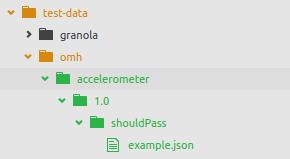
\includegraphics[width=0.5\textwidth]{imgs/newsampledata.png}
  \caption[Esquema de diretório para o novo sample]{Esquema de diretório para o exemplo do novo tipo de dados}
  
  \label{f:directorynewsample}
\end{figure}
  
\item Vamos agora preencher o ficheiro com a definição do novo tipo de dados, aquele que criou no ponto 2. O ficheiro vai ser criado no formato de \gls{JSON} schema. Para suportar a criação deste ficheiro pode reutilizar schemas existentes \cite{schema-library} e referênciá-los, deste modo estará a criar um modelo com tipos de dados normalizados. No meu caso vou reutilizar um schema para definir a data/hora e um outro para definir o tipo de atividade que está a efetuar no momento da leitura. Os restantes dados estão relacionados com o acelerómetro em si, a sessão e a leitura respetiva.
O ficheiro fica do seguinte modo: 

\begin{figure}[H]
\inputminted{json}{code/accelerometer-1.0.json}
\caption[\gls{JSON} schema para o novo tipo de dados de acelerómetro]{\gls{JSON} schema para o novo tipo de dados de acelerómetro}
\label{f:accelerometer-json-schema}
\end{figure}

\item Preencha o ficheiro com uma amostra do novo tipo de dados, para isso tem que ter em conta a definição utilizada, pois porque se esta amostra não for compatível não vai passar no validador.

\begin{figure}[H]
\inputminted{json}{code/example.json}
\caption[Exemplo do tipo de dados de acelerómetro]{Exemplo do tipo de dados de acelerómetro}
\label{f:accelerometer-json-data}
\end{figure}

\item Para compilar e executar o validador tem que executar o comando ''./gradlew test-data-validator:bootRun'' no diretório principal ''schemas'' ou então execute o comando ''./gradlew bootRun'' no diretório ''schemas/test-data-validator''. 

\subsection{Como utilizar o novo tipo de dados criado}

Para adicionar o novo tipo de dados criado, tem que o integrar com os restantes tipos de dados existentes. \par Tendo em conta que já tem o repositório omh-dsu-ri clonado através do comando ''git clone https://github.com/luistduarte/omh-dsu-ri', terá que copiar o seu novo tipo de dados para o diretório ''omh-dsu-ri/resource-server/src/main/resources/schema/omh'' que é onde se encontram os restantes tipos de dados válidos.

\end{enumerate}

\cleardoublepage
